\documentclass[10pt,a4paper,twoside,openright,titlepage]{book}
\usepackage[a4paper,top=3 cm ,bottom=3cm,left=4cm,right=3cm]{geometry}
\usepackage[T1]{fontenc}
\usepackage[utf8]{inputenc}
\usepackage[english]{babel}
\usepackage{amsmath,amssymb}
\usepackage{amsfonts}
  \newcommand{\overbar}[1]{\mkern 1.5mu\overline{\mkern-1.5mu#1\mkern-1.5mu}\mkern 1.5mu}
  \newcommand{\parallelsum}{\mathbin{\!/\mkern-4mu/\!}}
\usepackage{graphics}
\usepackage{graphicx}
\usepackage{sidecap}
\usepackage{textcomp}
\usepackage{subfig}
\usepackage{ulem}
\usepackage{soul} 
\usepackage{footnote}
\usepackage{lipsum}
\usepackage{setspace}
\usepackage[autostyle,italian=guillemets]{csquotes}
\usepackage[style=numeric,backend = biber]{biblatex}
\usepackage{guit}
  \addbibresource{bibliografia.bib}
\usepackage{frontespizio}
\usepackage{xcolor}
\definecolor{ruspa}{RGB}{0,102,0}
\usepackage[utopia]{quotchap}
\colorlet{chaptergrey}{ruspa}
%\usepackage{lmodern}

\usepackage{fancyhdr}
\renewcommand{\chaptermark}[1]{\markboth{#1}{}}
\renewcommand{\sectionmark}[1]{\markright{#1}}
\pagestyle{fancy}
\fancyhf{}
\fancyhead[LE,RO]{\thepage}
\fancyhead[LO]{\nouppercase{\rightmark}}
\fancyhead[RE]{\nouppercase{\leftmark}}
\renewcommand{\headrulewidth}{0pt}

\begin{document}

\begin{frontespizio}
  \Universita{Torino}
  \Logo[5cm]{logo}
  \Dipartimento{Fisica}
  \Corso{Fisica}
  \Annoaccademico{2015/2016}
  \Titolo{Study of the cluster shape in the upgraded silicon pixel detector of the ALICE experiment}
  \Candidato{Luca Barioglio}
  \Relatore{Prof. Massimo Masera}
  \NCandidato{Author}
  \NRelatore{Supervisor}{Supervisors}
  \Rientro{1cm}
  \Margini{2cm}{3cm}{2cm}{2cm}
\end{frontespizio}

\frontmatter
\newenvironment{abstract}%
    {\cleardoublepage\thispagestyle{empty}\null\vfill
    \begin{center}%
      \bfseries\huge\abstractname
    \end{center}}%
    {\vfill\null}
      \begin{abstract}
	ALICE (A Large Ion Collider Experiment) is designed for investigating the nature of the Quark-Gluon Plasma (QGP), a phase of deconfined strongly interacting matter, which occurs in extreme conditions of temperature (T $\sim$ 170 MeV) and baryo-chemical potential ($\mu B \sim$ 0).
	At the Large Hadron Collider, the QGP is obtained through collisions between beams of ultra-relativistic lead nuclei at $\sqrt{s_{NN}}$ = 5.02 TeV, with a collision rate of 8 kHz.\\
	The ALICE apparatus is designed to maximize the reconstruction of the tracks of the particles with low transverse momentum. In order to achieve this objective, detectors characterized by a low read-out rate are used for the Inner Tracking System (ITS). The current ITS configuration has a read-out of 1 kHz and  is not able to process all the Pb-Pb events.\\
	In 2020 there will be un upgrade of the LHC, which will translate in a higher luminosity and it will be possible to collide lead nuclei at the rate of 50 kHz. Thanks to this improvement, it will be possible to collect more statistics and, therefore, to study rare phenomena not accessible at the moment.\\
	For this reason, the ALICE experiment will undergo an upgrade as well, bringing the read-out rate from the current limit up to 50 kHz. In order to fulfill this request, there will be several changes in the detectors. In particular, the ITS, the closest detector to the interaction point and used for the tracking and the determination of the interaction point (vertexing), will be completely substituted.\\
	The ITS-upgrade will consist of seven cylindrical layers of silicon monolithic pixel sensors. These new sensors, characterized by a digital read-out system, have a maximum read-out rate of 100 kHz, making it possible to bear the interaction rate foreseen for the upgrade.\\
	The ITS-upgrade data are in the format of clusters of pixels, i.e. sets of adjacent fired pixels. Two kinds of information are associated to each cluster: its position within the matrix described by the pixels of the sensor and the cluster shape (topology), i.e. the pattern of fired pixels that constitutes the cluster itself.\\
	Starting from a cluster, an impact position with the relative error is needed: clusters with the same topology have the same impact position within the bounding box, i.e. the smallest rectangle containing the cluster itself, and the same related error.\\
	The information about the topology can be stored as a reference to a dictionary containing all the possible topologies, avoiding to store the whole bit-mask corresponding to the cluster shape and allowing to save storage space. Moreover, it is possible to avoid to compute information concerning the topology each time a cluster with a specific topology is found.\\
	Furthermore, Monte Carlo simulations show that the frequency distribution of the topologies is highly not uniform. For this reason, data can be compressed using the Huffman coding, a compression algorithm based on the relative frequency of characters, in this case topologies, which associates the shortest string to the most common character, reducing the storage space needed.\\
	However, the Huffman coding needs to work with at most few thousands of different characters in order to be efficient and for this reason the number of topologies in the dictionary must be reduced. This reduction can be done by grouping rare topologies with similar mean characteristics, in order to reduce the number of entries in the dictionary at the expense of a loss of details about rare instances.\\
	Therefore, the main aim of my thesis work is the development of an algorithm for the creation of a dictionary, containing the information of the common topologies and of the groups of rare topologies. Then, another aim of my project is the implementation of the algorithm for the identification of a topology with the corresponding key in the dictionary, in a time compatible with the read-out rate.\\
      \end{abstract}

\onehalfspacing
\tableofcontents

\mainmatter
\chapter{High Energy Nuclear Physics}
%
In this first chapter a basic description of the physics of strongly interacting matter, in particular of the properties of the Quark-Gluon Plasma (QGP) and of the main observables from which it is possible to characterize it, is given, in order to introduce the reader to the theoretical framework of the relativistic heavy-ion physics.
%
\section{QCD}
Within the Standard Model, the Quantum Chromodynamics (QCD) is the gauge theory describing the colour interaction between quarks and gluons. This theory is based on the non-abelian group $SU(3)_{C}$, whose generators are the eight Gell-Mann matrices ($\lambda^{a}$, with $a=1,...,8$). A vector boson (gluon) is associated to each generator and the algebra of the group determines the interaction vertices.\\
The QCD lagrangian is given by equation:
%
\begin{equation}
 \label{lQCD}
 \mathcal{L}_{QCD} = \overbar{\psi}(i\gamma^{\mu}D_{\mu}-m)\psi - \frac{1}{4} G^{a}_{\mu\nu}G_{a}^{\mu\nu}
\end{equation}
%
with
%
\begin{equation*}
  D_{\mu} = \partial_{\mu} - i g \, \frac{\lambda_{a}}{2} \, A^{a}_{\mu}(x)
\end{equation*}
%
and
%
\begin{equation*}
  G^{a}_{\mu\nu}(x)=\partial_{\mu}A^{a}_{\nu}(x)-\partial_{\nu}A^{a}_{\mu}(x)+ g f_{abc} A^{b}_{\mu}(x)A^{c}_{\nu}(x)
\end{equation*}
%
Since the group $SU(3)_{C}$ is non abelian, i.e. the structure constants $f_{abc}$ are not null, interactions between gauge bosons are allowed, in particular vertices with three and four gluons can be found, making QCD extremely different than QED: first, gluon are colour-charged, second, strong interaction is low range.

\subsection{Running coupling constants}

Many aspects of strong interaction can be explained considering the coupling constant $\alpha$ as a function of the energy scale: this dependence is due to the renormalization scheme of the adopted perturbative framework.\\
QED case will be first considered in order to let a better comprehension of the problem.\\
From the renormalization theory, the QED coupling constant as a function of $Q^{2}$ is given by equation:
%
\begin{equation}
  \alpha(|Q|^{2})= \frac{ \alpha(\mu^{2})}{1-\frac{\alpha(\mu^{2})}{3\pi}ln(|Q|^{2} / \mu^{2})}
  \label{eq:aqed}
\end{equation}
%
where $\mu$ is the energy scale used to fix the overall scale constant, which cannot be determined by the theory.\\
This behaviour can be explained by the analogy with a negative charge immersed in a dielectric medium: as in the case of the dielectric the negative charge polarizes the molecules of the medium, orienting the positive charges towards the negative one, causing its screening, likewise the presence of a charge in the vacuum causes the polarization of the virtual electron-positron couples and a screening of the electric charge itself. For this reason, the screening is greater at long distances and the value of the charge, then of $\alpha$, increases as the distance decreases, or rather as the transferred momentum increases, as shown in Figure \ref{qedalpha}.
%
\begin{figure}
  \centering
  \subfloat[][]
  {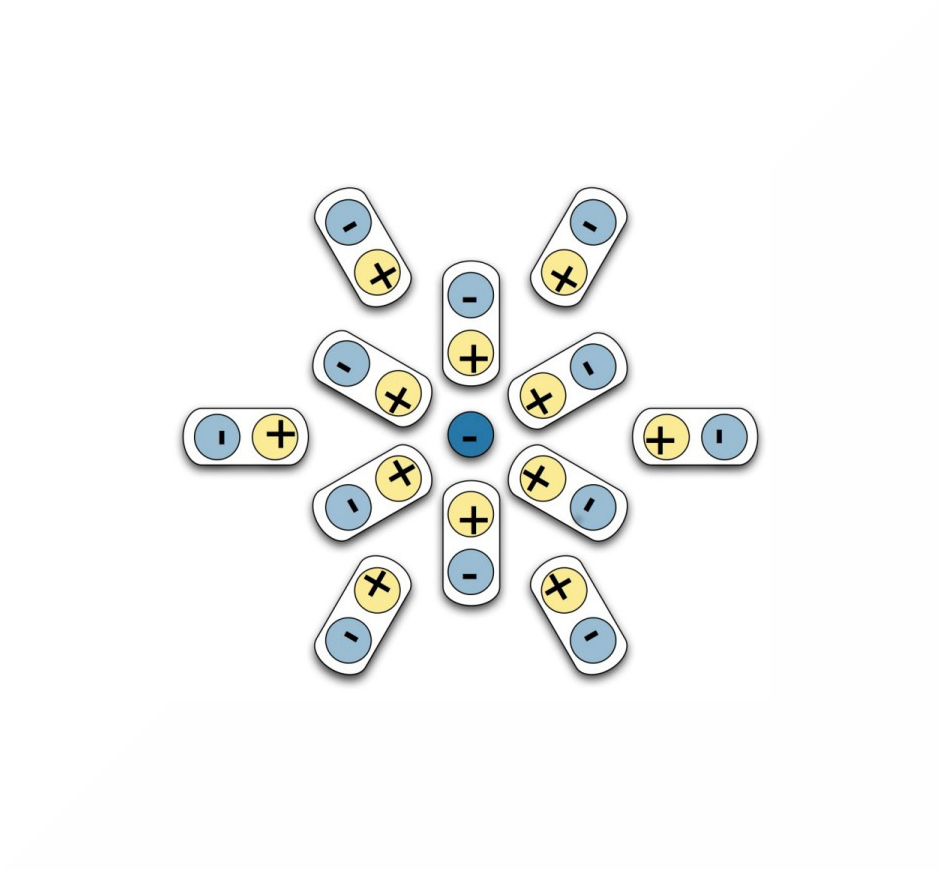
\includegraphics[scale=0.22]{figures/pol.jpg}\label{pol}}\quad
  \subfloat[][]
  {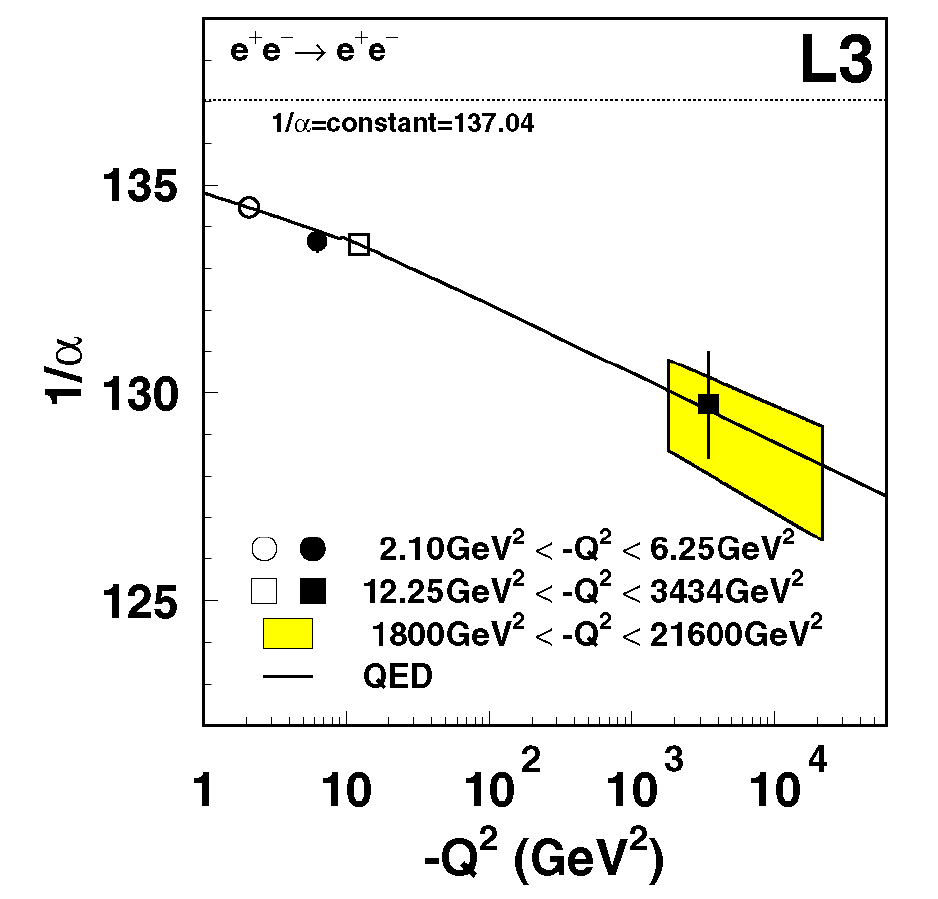
\includegraphics[scale=0.25]{figures/qedalpha.png}\label{qedalpha}}
  \caption{(a) Example of polarization (b) Measurement of the running of the electromagnetic coupling as a function of momentum-transfer at LEP \cite{achard2005}.}
\end{figure}
%
In QCD, instead, the coupling constant $\alpha_{S}$ has a different behaviour, due to the fact that there are gluon loops besides fermion loops. Indeed the renormalization theory shows that bosonic and fermionic loop contributions have opposite signs: besides the screening of the colour charge, like for electric charge in QED, there is an antiscreening effect due to gluon loops.\\
The evolution of the strong coupling constant is given by equation:
%
\begin{equation}
 \alpha_{S}(|Q|^{2})= \frac{ \alpha_{S}(\mu^{2})}{1+\frac{\alpha_{S}(\mu^{2})}{12\pi}(33-2n_{f})ln(|Q|^{2} / \mu^{2})}
 \label{eq:aqcd}
\end{equation}
%
where $n_{f}$ is the number of the quark flavours effectively contributing to the loops, namely those with mass $m_{f} < |Q|$.
%
\begin{figure}
  \centering
  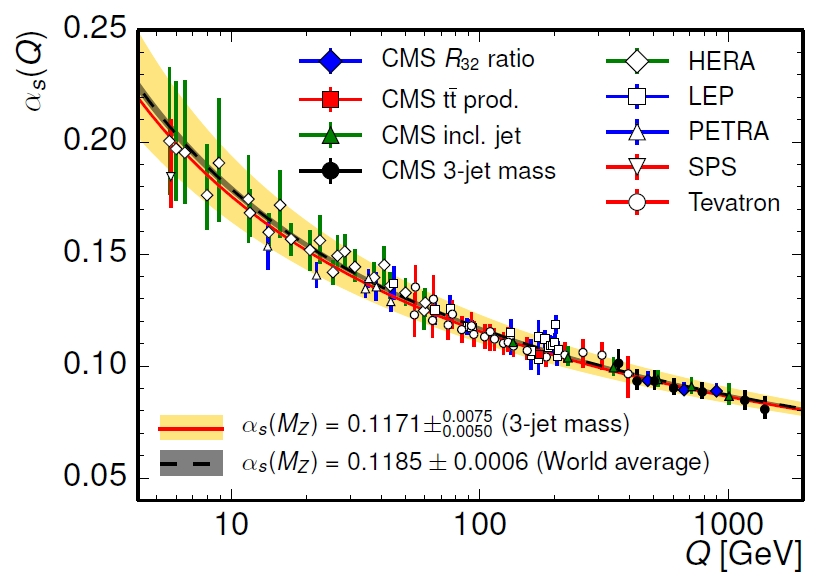
\includegraphics[scale=0.30]{figures/alphas_3j.jpg}
  \caption{Calculations and measurements of strong coupling constant $\alpha_{S}$ as a function of the energy scale Q \cite{kh2015}.}
  \label{fig:alphas}
\end{figure}
%
The value of $\alpha_{S}$ as a function of the energy scale Q can be seen in Figure \ref{fig:alphas}: it decreases when the transferred momentum increases, i.e. when the distance decreases. In particular, for small values of $Q^{2}$ the coupling constant assumes large values and the perturbative approach is not possible anymore.
For this reason, it is convenient to introduce the parameter $\Lambda_{QCD}$, which represents the limit energy scale for the perturbative approach. Using $\Lambda_{QCD}$ equation \ref{eq:aqcd} can be rewritten for large values of the transferred momentum ($|Q|^{2} \gg \Lambda^{2}$) as:
%
\begin{equation}
 \alpha_{S}(|Q|^{2})= \frac{12\pi}{(33-2n_{f})ln(|Q|^{2} / \Lambda^{2})}.
 \label{eq:aqcd2}
\end{equation}
%
For the above considerations, two regimes can be distinguished: asymptotic freedom and confinement.\\
Asymptotic freedom is the regime of high energy, where the coupling constant $\alpha_{S}$ is small enough to allow a perturbative approach: for $Q \sim$ 100 GeV - 1 TeV, $\alpha_{S}$ is about 0.1. For such energies the strong interaction becomes mild, reducing the energy necessary to divide colour charges and to release quark and gluons from their bound states. Since high $Q^{2}$ means short distances, it is possible to obtain this state of free partons by compressing or heating QCD matter: the result is a plasma of quark and gluons, the QGP, of which it will be discussed in the next section.\\
Confinement, instead, is the regime of low energy, where the perturbative approach is not valid anymore but other theoretical methods can be used, like, e.g., lattice QCD. In this range of energy, as already said before, the strong interaction becomes more important thanks to the formation of gluon loops and to the consequent antiscreening of the colour charges. Moreover, the energy necessary to separate two colour charges increases with the separation itself, making the system move towards a stable equilibrium characterized by the absence of free colour charges and by the formation of colourless states. Two methods used for the study of confined will be discussed in the next section.

\clearpage

\section{QCD phase space diagram}
%
\begin{figure}
  \centering
  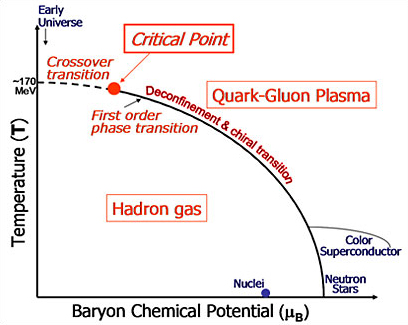
\includegraphics[scale=0.5]{figures/phase.jpg}
  \caption{Phase diagram for strongly interacting matter}
  \label{fig:phase}
\end{figure}
%
Nuclear matter is expected to exhibit different behaviours depending on its temperature T and baryo-chemical potential $\mu_{b}$. The latter is defined
as the energy needed to increase by one unity the total number of baryons and anti-baryons, $\mu_{B}= \partial E / \partial N_{B}$, and is related to the baryon density. An example of phase diagram is given in Figure \ref{fig:phase}.\\ At low temperatures and small $\mu_{B}$ ($\sim$1 GeV), nuclear matter is confined in hadrons and atomic nuclei. A state of hadronic gas can be reached either by increasing T or compressing the nuclear matter, i.e. increasing $\mu_{B}$: in these conditions, the nucleons can interact and form pions, excited states or other hadrons.
For even larger values of T and $\mu_{B}$ the transition to the phase of QGP, a state of deconfined strongly interacting matter, is predicted. These conditions necessary to the formation of QGP existed in the very first stages of the Universe: in facts, according to the Big Bang theory, about fourteen billion years ago the Universe was concentrated in a very small region of space, characterized by almost infinite temperature and energy, and then it started expanding and consequently cooling down. In the first stages, corresponding to few microseconds after the Big Bang, the temperature was so high that hadrons could not be formed and all the strongly interacting matter existed in form of QGP. However, for the expansion and the cooling, the energy density and the temperature of the Universe decreased under critical values, respectively $\epsilon_{c}\approx1 \;$GeV$/fm^{3}$ and $T_{c}\approx 170\; $MeV $ \approx 2\cdot10^{12}\; K$, for which a state of deconfined matter was not possible anymore, causing the transition to a confined state.\\ Unfortunately, it is not possible to observe the characteristics of this primordial state, since the transition from deconfined to confined matter took place when the electromagnetic radiation was still coupled with the primordial plasma constituting the universe, which therefore was opaque. For this reason, the only way to study the characteristics of the QGP, and of the transition from this to the hadronic phase, is to recreate these conditions using high energy heavy ions collisions, as it will be seen farther.
However, in orther to describe the evolution of QGP and, above all, the hadronization, it is not possible to use the perturbative approach for the reason said before and some methods to describe confined strongly interacting matter are needed.

\subsection{MIT bag model}

The MIT bag model is an effective model that describes, in a phenomenological way, quarks and gluons confined within the hadrons. Even if based on very simple hypothesis, the MIT bag model allows to give a description of confinement and phase transition, giving rough estimations of the critical temperature $T_{C}$, corresponding to the transition from deconfined to confined strong interacting matter. In the MIT bag model quarks are seen as massless fermions inside a spherical bag of finite dimensions, whose confinement is due to the balance between the pression exerted from the particles on the bag, coming from their kinetic energy, and an external pressure \textit{ad hoc} introduced, which takes into account effects that cannot be calculated through a perturbative approach. Considering these hypotheses, it is possible to evaluate the pressure on the bag for a confined state.\\
The equation of motion for a massless fermion is the Dirac equation:
%
\begin{equation}
  \gamma^{\mu}p_{\mu}\psi=0
\end{equation}
%
Imposing the confinement conditions means that on the surface of the bag the scalar density must be null:
%
\begin{equation}
  \overbar{\psi}\psi \Big|_{bag} = 0 \ \ \ \longrightarrow \ \ \ E = \frac{2.04 \hbar c}{R},
\end{equation}
%
where R is the radius of the bag.\\
Calling B the external pressure on the bag, the total energy of the system is equal to:
%
\begin{equation}
  E = \frac{2.04N \hbar c}{R} + \frac{4}{3} \pi R^{3} B,
\end{equation}
%
being N the number of particles within the bag.\\
From this equation, the radius of the bag and the external pressure B can be determined imposing the equilibrium condition, in other words minimizing the energy:
%
\begin{equation}
  \frac{dE}{dR} = -\frac{2.04 \hbar c}{R^{2}} + 4 \pi R^{2} B = 0 \ \ \ \longrightarrow \ \ \ B^{\frac{1}{4}} = \frac{\hbar c}{R}\Big(\frac{2.04N}{4\pi}\Big)^{\frac{1}{4}}
\end{equation}
%
Considering a baryon composed of three valence quarks, with a radius of 0.8 fm, the value of the fourth root of the external pressure is $B^{\frac{1}{4}} = 206 \; $MeV$ / (\hbar c)^{3/4}$. In this way, the effects of non perturbative QCD are included in the external pressure B, expressly introduced for this reason, and this pressure is balanced from the internal pressure exerted by the quarks. According to the MIT bag model, the phase transition can be seen as the increase of the internal pressure to the point at which it overcomes the external one, giving birth to a new phase in which quarks are no more confined within hadrons, but free to move in a bigger volume: the state of QGP is therefore enhanced.\\
The internal pressure can increase in two ways: by compression, i.e. increasing the baryonic density, or by increasing the temperature, i.e the kinetic energy of the quarks. Focusing on the latter, it is possible to obtain the temperature at which the phase transition occurs, requiring the external pressure to match the internal one: 
%
\begin{equation}
  P = 37 \frac{\pi^{2}}{90}T^{4}_{C} = B \ \ \ \longrightarrow \ \ \ T_{C} = \Big(\frac{90B}{37\pi^{2}}\Big)^{\frac{1}{4}}= 145 \ MeV
\end{equation}
%
As far as concerns the MIT bag model, a transition from nuclear matter to QGP is expected at $T_{C} = 145$ MeV. However, as already said, this result comes from simple hypotheses and, for this reason, a more precise result can be obtained using more sophisticated methods, such as lattice QCD, which will be discussed in the next section.\\

\subsection{Lattice QCD}
%
Lattice QCD is the main tool to study non-perturbative aspects of QCD and is based on the discretization of the space-time, treated, indeed, as a lattice. This theory offers important advantages: first of all, if in the perturbative approach there is the problem of the divergence of the integrals with respect to the momentum for large values of this, which can be solved using a renormalization method, in lattice QCD this problem does not exist because the pitch of the lattice defines a minimum distance and consequently a cut-off value for the momentum. Then, the lattice partition function can be written as a path integral and, therefore, easily calculated, for example using Monte Carlo methods. On the other hand, the computational cost of numerical simulations can increase dramatically as the lattice spacing decreases, causing a constrain on the minimum pitch to use for the calculations. Moreover, in order to reduce the computational burden, further approximation are needed. For example, one of the most common approximation is the so called \textit{pure gauge}, in which quarks are considered as static sources of the colour field, fixed in the knots of the lattice, that is equivalent to considering the masses of the quarks infinite. Corrections to include the finite masses of the quarks and a not-null baryo-chemical potential are possible but under development.\\
In order to explain the basics of lattice QCD, the quantum mechanics case will be first considered for simplicity; then, it will be extended to quantum field theory.
The grand canonical partition function of the system at a temperature T can be written as:
%
\begin{equation}
 Z = \sum\limits_{x_{a}}\langle x_{a} | e^{-\beta T} | x_{a} \rangle
\end{equation}
%
where the sum is over all the possible states $x_{a}$ of the system, $\beta=1/T$, and H is the hamiltonian operator.\\
This formula is very close to Feynman path integrals:
%
\begin{equation}
 \langle x_{b} | e^{- i H (t_{b} - t_{a})} | x_{a} \rangle = \int \prod\limits_{i=1}^{n_{t}-1} dx_{i} e^{i S_{M}(x_{a},x_{1},\dots,x_{n_{t}-1},x_{b})}
\end{equation}
where $x_{a}$ and $x_{b}$ are initial and final position, respectively at time $t_{a}$ and  $t_{b}$, $x_{i}$ is any of the $n$ intermediate positions in which it has been decided to divide the path and $S_{M}$ is the minkowskian action.\\
The two previous expressions are very alike, but there are few differences and, for this reason, in order to express the partition function as a path integral, some precautions are needed. First of all, the exponent of the former is real, while the one of the latter is imaginary: it can be solved using a change of variable $t = -i \tau$, known as \textit{Wick rotation}, that is equivalent to using an imaginary time and passing from a minkowskian to an euclidean action. Then, in the partition function formula, initial and final states are the same: this problem can be solved imposing periodic boundary conditions, i.e. $x(\tau_{b}) = x(\tau_{b})$. Choosing appropriate $\tau$ boundaries, i.e. $\tau_{a} = 0 \leq \tau \leq \tau_{b} = \tau_{n_{t}}$, the previous condition can be written as $x_{a} = x(\tau_{n_{t}})$ and the expression for Z becomes:
%
\begin{equation}
 Z = \int dx_{n_{t}} \prod\limits_{i=1}^{n_{t}-1}dx_{i} \; e^{iS_{M}\Big|_{t=-i\tau}} = \int \prod\limits_{i=1}^{n_{t}}dx_{i} \; e^{-S_{E}} \equiv \int \mathcal{D}x \; e^{-S_{E}(x)}
\end{equation}
%
The last step is the extension to the quantum field theory:
%
\begin{equation}
 Z = \int \mathcal{D}\phi(x,\tau) \; e^{-S_{E}(\phi(x,\tau))}
\end{equation}
%
The most efficient numerical approach to calculate path integrals is to estimate thermal averages over specific paths, which are identified using Monte Carlo algorithms of importance sampling. Then, the path integrals are evaluated introducing a four-dimensional space-time lattice, whose spacing is the smallest permitted by the computational limits.\\
As already said before, using lattice QCD it is possible to get more precise prediction about the phase transition, but its characteristics are, for example, strongly dependent on the treatment of quark masses and precise calculations are available only in the limit of vanishing baryo-chemical potential ($\mu_{B}\sim0$). In particular, in the limit of two quarks flavours with null mass, a second-order transition is predicted, while a first-order one is foreseen in case of three massless quarks. However, recent calculations of lattice QCD predict a critical an estimated temperature $T_{C}\approx160$ MeV, corresponding to an energy density $\epsilon_{C} = 0.7 \pm 0.3$ GeV$/fm^{3}$\cite{lattice}.

\section{Heavy ions collisions}
In order to study the properties of the QGP, it is necessary to create a system of strongly interacting matter at extreme conditions of temperature and energy density, which could be described using the thermodynamics. For this reason, this system should be characterized by a wide spatial extension, so that it could be described using macroscopic variables, such as the temperature or the pressure. Therefore, first, the system must have an extension which must be much greater than the strong interaction scale ($\sim$ 1 fm); then, it must be characterized by a great number of particles (high multiplicity). Furthermore, the system must be long lived, so that a high number of collisions between the constituents can occur and lead to thermal equilibrium, necessary for using a thermodynamic approach. The thermal equilibrium is reached when the free mean path of the constituents ($\tau_{path}$) is greater than the system dimension and smaller than the life time of the system ($\tau_{system}\gg\tau_{path}$). These hypothesis has to be verified comparing the theoretical prediction with the experimental data. However, in high energy nucleus-nucleus collisions, all these requirements are expected to be fulfilled, thanks to the multiple collisions between nucleons of the colliding nuclei. In facts, a nucleon collides with many nucleons in the other nucleus, releasing energy. For this reason, there is a large energy deposit in the interaction region, determining a high energy density of the system and, therefore, a high temperature. Moreover, a large number of primary particles is produced, determining the high multiplicity required as hypothesis.\\
In the next sections, it will be shown how to describe nucleus-nucleus collisions and how this kind of events evolves.\\

\subsection{Glauber Model}
The Glauber Model provides a description of the nucleus-nucleus interaction as an incoherent superposition of nucleon-nucleon collisions.
The key element of the Glauber model is the impact parameter $\vec{b}$, a geometrical parameter defined as the distance between the centres of the two nuclei in the transverse plane. The impact parameter is important because it determines the centrality of the collision. Central collisions are characterized by a small impact parameter: in this kind of events many nucleons are involved in the interaction and, therefore, there are many collisions between nucleons and many particles are produced. Peripheral collisions, instead, are characterized by a large impact parameter: the overlap region is smaller and so there are few nucleons involved in the interaction, hence few collisions between nucleons and few particles produced.\\
The Glauber Model is based on few assumptions, also known as \textit{optical limit}:
\begin{itemize}
 \item the nucleons are point like;
 \item the nucleons inside the nuclei are independent;
 \item the nuclei, hence the constituent nucleons, travel in a straight line: there are no deflections;
 \item only the strong interaction is considered: protons and neutrons cannot be distinguished;
 \item the cross section for an elementary nucleon-nucleon interaction is the same for all the passage of the nucleon through the target.
\end{itemize}
During the collisions we can distinguish two kinds of nucleons: the spectators are those nucleons that do not interact with any nucleon of the other nucleus; the participants are the nucleons which have interacted at least with a nucleon of the other nucleus.\\
Even if this model is based on simple hypotheses, it allows to get much information, such as the probability of interaction, the number of elementary collisions, the number of participant nucleons, the number of spectators, etc.
%
\begin{figure}
  \centering
  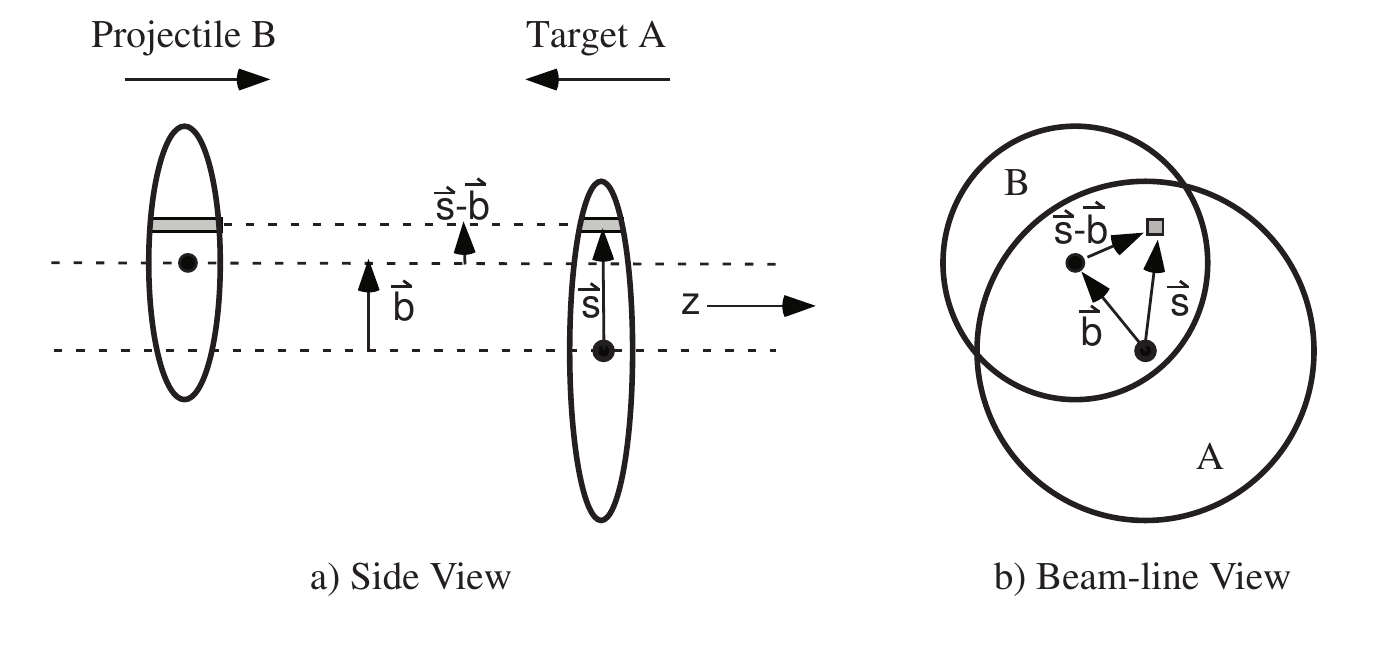
\includegraphics[scale=0.30]{figures/Impact_parameter.png}
  \caption{Schematic view of a nucleus-nucleus collision in the longitudinal (a) and transverse (b) plane.}
  \label{fig:impact}
\end{figure}
%
\subsection{Rapidity and Pseudorapidity}
Before describing the evolution of a nucleus-nucleus collision, it is necessary to introduce two important variables, essential for the description of these phenomena: the rapidity \textit{y} and the pseudorapidity $\eta$.\\
The rapidity is the parameter that arises in the linear representation of a Lorentz boost:
\begin{equation}
 \left(
    \begin{array}{c}
      E'\\
      p'_{\:\parallelsum}
    \end{array}
  \right) = 
      \begin{pmatrix}
      \cosh y & \sinh y \\
      \sinh y & \cosh y 
    \end{pmatrix}
  \;
  \left(
     \begin{array}{c}
      E\\
      p_{\:\parallelsum}
    \end{array}
  \right)
\end{equation}
%
From this equation, it can be easily shown that the rapidity, assuming a Lorentz boost along z direction, which is the beam direction, can be expressed as:
\begin{equation}
 y = \frac{1}{2}\ln\frac{E + p_{z}}{E - p_{z}}
\end{equation}
However, from an experimental point of view, the determination of the rapidity requires the identification of the particle, which, in certain cases, could be very difficult, or the measurement of two different quantities, such as $E$ and $p_{z}$. Therefore, this variable is often substituted by the pseudorapidity $\eta$, which is related uniquely to the polar angle $\theta$ by the expression:
\begin{equation}
 \eta = \frac{1}{2}\ln\frac{|\vec{p}\:| + p_{z}}{|\vec{p}\:| - p_{z}} = - \ln [\tan (\theta/2)]
\end{equation}
In the high energy limit, it can be shown that $\lim_{\beta \to c} \eta \;= \;y$.\\
These two parameters are extremely important, since many variables, like, for example, the multiplicity, are described in terms of rapidity or pseudorapidity.\\


\section{Evolution of nucleus-nucleus collisions}
The collision between two ultra-relativistic nuclei is an event characterized by a complex space-time evolution: a scheme of this process can be found in Figure \ref{fig:evol}.\\
Before the collision takes place, the two nuclei travel along the beam direction at a speed close to the speed of light and, for this reason, they are Lorentz-contracted. This means that the two nuclei can be represented as two disks.\\
At $t=0$, the two nuclei collide, hence scatterings between the nucleons of the projectile and of the target take place. In each of this collision, the nucleons lose energy ad momentum and, in case of inelastic scattering, they could become unstable baryon-like objects. Withal, at the LHC energies, after the interactions these products still have enough energy to escape the interaction region, which, in the case of a symmetric collider such as the LHC, is the mid rapidity region ($y\sim0$), and decay far away from this region. Therefore, for high energy collisions, the mid-rapidity region is characterized by a high energy density, with the generation of $q\bar{q}$ pairs, but with a low baryonic content, i.e. a vanishing baryo-chemical potential ($\mu_{B}\sim$ 0). All together these conditions form the so called \textit{transparency regime}. The transparency regime is characterized by a large number of particle for unity of rapidity ($\frac{dN}{dy}$) in the mid rapidity region. Therefore, in these distributions a plateau around $y\sim0$, whose width and height is determined by the energy of the collision, is expected.\\
If the temperature of the medium created is larger than a critical value $T_{C}$, the formation of a system of deconfined quarks and gluons is expected. The QGP could be initially not in thermal equilibrium but, thanks to the high number of scatterings, it should thermalize at a proper time $\tau_{0}$, whose value strongly depends on the centre of mass energy of the experiment. At the LHC energies, for example, $\tau_{0}<$ 0.2 fm/c. After $\tau_{0}$, the system is expected to evolve according to the hydrodynamics: the plasma expands and for this reason the temperature decreases until it reaches the critical value $T_{C}$ and the process of hadronization starts. In case of first order transition, the system is characterized by a mixed phase, where the QGP coexists along with confined hadronic matter. This mixed phase lasts for a time $\tau\sim$ 10 fm/c, after which the system appears as a gas of hadrons, in which a large number of scatterings, both elastic and inelastic, can take place.
When the temperature reaches values for which the inelastic scatterings are not possible anymore, the chemical composition is fixed: this moment is called chemical freeze-out and occurs at a temperature $T_{ch}$. After the chemical freeze-out, the system continue expanding and the elements interact via elastic scatterings until the temperature drops below the vale $T_{kin}$, at which the thermal freeze-out occurs. After the thermal freeze-out, the hadrons finally stream out of the collision region. Typical values of the chemical and thermal freeze-out temperatures, estimated at the LHC in central Pb-Pb collisions at $\sqrt{s_{NN}} =$ 2.76 TeV, are $T_{ch}\sim$ 160 MeV and $T_{kin}\sim$ 100 MeV \cite{temp}.
%
\begin{figure}
  \centering
  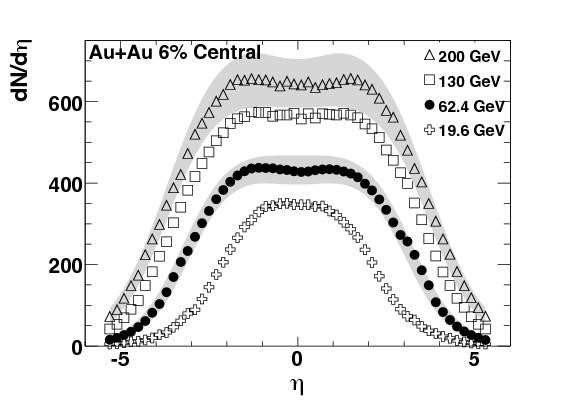
\includegraphics[scale=0.5]{figures/dNdeta.png}
  \caption{Charged particle multiplicity distributions for collisions at RHIC with four different energies as a function of pseudorapidity\cite{dndeta}.}
  \label{fig:dndeta}
\end{figure}
%
%
\begin{figure}
  \centering
  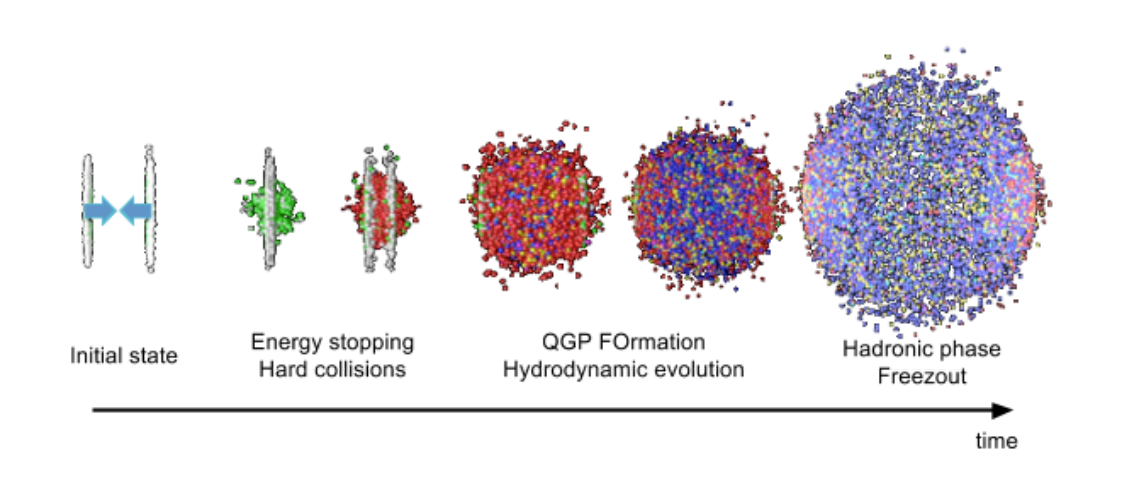
\includegraphics[scale=0.5]{figures/evolution.png}
  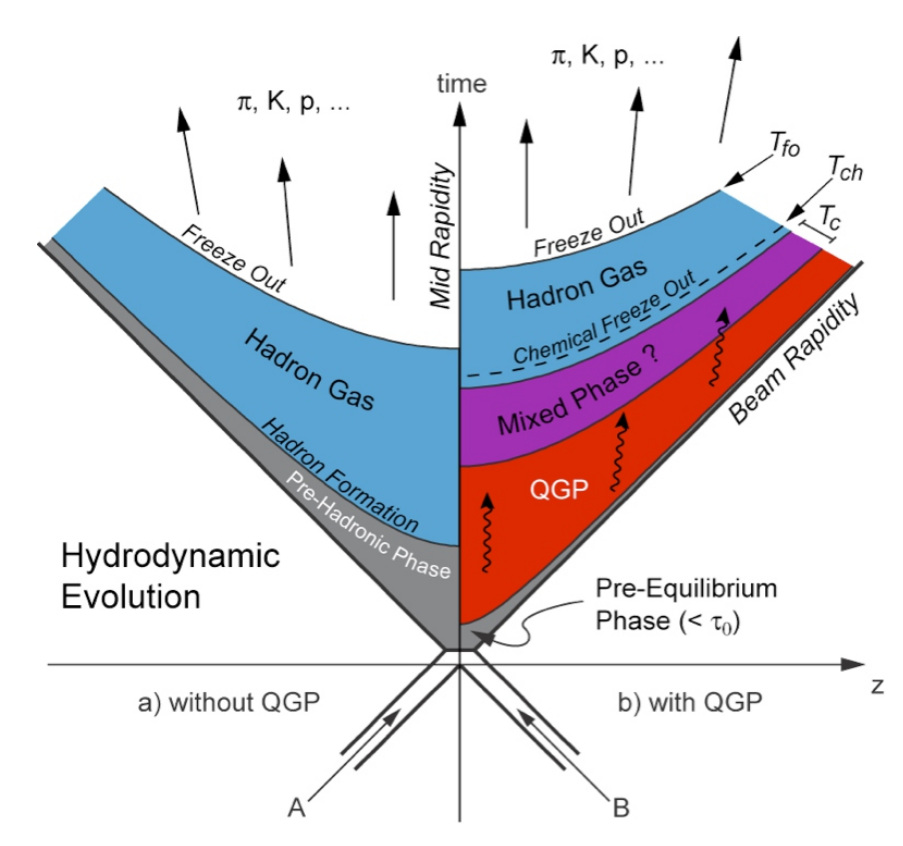
\includegraphics[scale=0.35]{figures/spacetime.png}
  \caption{Space-time evolution of a collision between nuclei, described with a hydrodynamic approach.}
  \label{fig:evol}
\end{figure}
%
\clearpage
\section{Experimental observables in ALICE}
Since the QGP, from an experimental point of view, is characterized by a short life time (few $10^{-23}$ s), the direct measurement of variables such as, for example, temperature, is not possible. Indeed, the only accessible variables are those that characterize the final state, i.e. those related to the particles present in the last stage of the collision process, as previously described. For this reason, the theoretical models are extremely important to define which characteristics of the final state could provide information about the QGP formation and the phase transition. In facts, comparing the experimental measurements with the theoretical predictions, it is possible to indirectly determine important quantities, which are parameters of the theoretical models, related to stages of the evolution of the system otherwise not accessible.\\
These quantities can be measured considering different kinds of probes: electroweak probes and hadronic probes. The formers (dielectrons and direct photons) are related to the early stages of the evolution of the fireball. In facts, they do not interact strongly and so they can pass through the generated medium unharmed. However, they are less abundant then the hadronic probes and, concerning the direct photons, it is difficult to divide these from the background generated in the following stages. The hadronic probes, otherwise, are more abundant but are influenced by the medium and by the final state effects. Consequently, it is difficult to distinguish particles produced in the earliest stages of the collision from those generated in later stages or in hadronic processes.\\
It is also possible to make another distinction among the probes, according to the value of the transferred momentum of the process in which they have been generated.\\
The hard probes are produced in the first stages of the collision, when the energy of the system has not degraded yet, in processes characterized by a high momentum transfer, like, for example, the interaction between high momentum partons. They are rare processes, whose number scales with the number of collisions among the nucleons constituting the projectile and the target nuclei, and are sensible to the following stages of the collision. The soft probes, instead, are produced in the last stages of the collisions, by processes characterized by a low momentum transfer. For this reason, they cannot resolute the the partonic structure of the nucleons. However, even if they are produced during the hadronic stage, they keep indirect information on the properties of the phase transition and on the QGP. Then, the soft probes constitute the bulk of the hadrons produced in the collision, above the 99$\%$.\\
In the next sections, the most important observables for ALICE will be described.\\
\subsection{Particle multiplicity}
The multiplicity is the number of particles produced in a collision. Two kinds of multiplicity measurements can be distinguished: the multiplicity of not identified particles, i.e. the total number of particles produced, and the multiplicity of identified particles, i.e. the number of particles of a certain species.
\subsubsection{Multiplicity of not identified particles}
In the study of the collisions between nuclei, this quantity is extremely important, since it gives information about the centrality of the collision, the energy density of the final state and the mechanisms of particles production. Moreover, it is also an important parameter for the design of an experiment for the study of ions collisions, since the occupancy of the detectors is closely related to the density of particles, hence to the multiplicity. Similarly, the radiation damage is related to the flow of the particles through the detectors and the readout electronics. As far as concerns the ALICE experiment, this was designed to run with multiplicity up to 8000 particles per unit of rapidity in the mid-rapidity region. However, this estimation was made in a period when RHIC multiplicity data were not available and happened to be overestimated, since the measured value is approximately 1600 charged particles per rapidity unity\cite{mult}.\\  
As mentioned before, the multiplicity is related to the centrality of the collision, i.e. to the value of the impact parameter. In facts, for the Glauber Model, both the number of elementary collisions and the number of participant nucleons are related to the impact parameter. Since in each elementary collision there is a release of energy, each collision contributes to the production of particles, then to the multiplicity. Typically, the measure of the total cross section per charged particle as a function of the charged multiplicity is used to express the centrality, as shown in Figure \ref{fig:centr}: it is expressed as the percentage of area under curve.\\
%
\begin{figure}
  \centering
  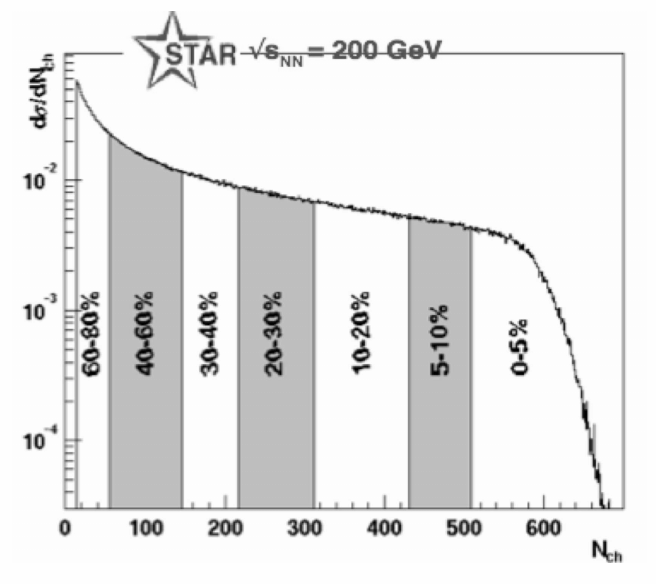
\includegraphics[scale=0.5]{figures/star.png}
  \caption{A typical event multiplicity distribution at RHIC, sliced up in centrality classes.}
  \label{fig:centr}
\end{figure}
%
Then, the measurement of the charged multiplicity per pseudorapidity unity at mid-rapidity allows an estimation of the energy density of the QGP, using a method proposed by Bjorken.\\
According to this method, in the frame in which both the colliding nuclei have high energy, the projectile and the target, that are Lorentz contracted, can be seen as two disks that rapidly pass through each other. Then, secondary particles are generated in this region bounded by the two disks, which is characterized by a low longitudinal extension. A scheme of this model can be seen in Figure \ref{fig:bjor}.\\
%
\begin{figure}
  \centering
  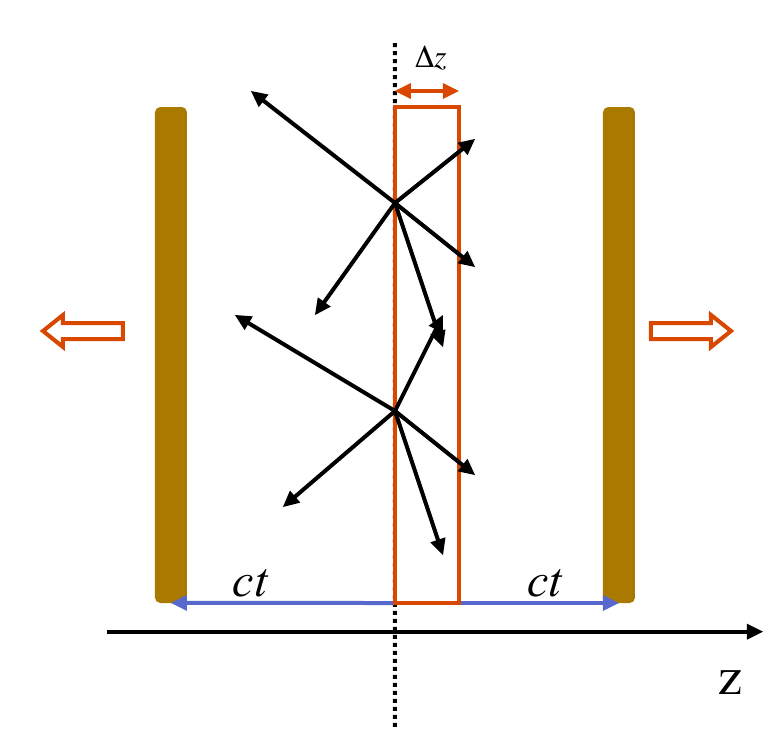
\includegraphics[scale=0.3]{figures/bjorken.png}
  \caption{A scheme of Bjorken's model for the collision between high energy nuclei.}
  \label{fig:bjor}
\end{figure}
%
According to these hypotheses, the mid-rapidity region is characterized by a certain number of particles that have formed at a time $\tau_{0}$. It is possible to determine the energy density of this region at the time of formation of these secondary particles, considering the region of longitudinal width $\Delta z$ and transverse section \textit{A} shown in Figure \ref{fig:bjor}. This region includes all the particles with a longitudinal speed in the range 0 $\leq \beta_{z} \leq \frac{\Delta z}{\tau_{0}}$. Therefore, the number of particles within this region is given by the expression:
\begin{equation}
 \Delta N \;=\; \int_{0}^{\frac{\Delta z}{\tau_{0}}} \frac{dN}{d\beta_{z}}d\beta_{z}\;\cong\;\frac{\Delta z}{\tau_{0}}\frac{dN}{d\beta_{z}}\;=\;\frac{\Delta z}{\tau_{0}}\frac{dN}{dy},
\end{equation}
where in the last passage the approximation $\beta_{z}\sim y$ has been done, since the rapidity is almost null. Then, since the rapidity is close to zero, the energy of the particles coincides with their transverse mass $m_{T} = \sqrt{m_{0}^{2} + p_{T}^{2}}$, since $E = m_{T} \cosh y \cong  m_{T}$. Hence, the average energy density of this region is:
\begin{equation}
 \langle \epsilon(\tau_{0}) \rangle \; = \; \frac{\Delta N\langle m_{T}\rangle}{\Delta z\:A}\;=\;\frac{\Delta z}{\tau_{0}}\frac{dN}{dy}\frac{\langle m_{T}\rangle}{\Delta z\:A}\;=\;\frac{1}{\tau_{0} A} \langle m_{T} \rangle \frac{dN(\tau_{0})}{dy}\;=\;\frac{1}{\tau_{0} A}\frac{dE_{T}(\tau_{0})}{dy},
\end{equation}
where $E_{T}$ is the transverse energy and \textit{A} is the area of the overlapping region.\\
Summing up, at mid-rapidity the energy density can be determined using the Bjorken's formula:
\begin{equation}
 \epsilon_{Bj}\;=\; \frac{1}{\tau_{0} A}\frac{dE_{T}}{dy}\Big|_{y=0}\;\sim\;\frac{1}{\tau_{0} A}\langle E_{T} \rangle \frac{dN}{d\eta}\Big|_{\eta=0}
\end{equation}
Measuring the pseudorapidity density $\frac{dN}{d\eta}$ and the average hadron energy transverse energy $\langle E_{T} \rangle$, which can be obtained experimentally by measuring the energy of charged hadrons, if an estimation of the time of formation $\tau_{0}$ is given, the energy density can be easily determined. ALICE obtained for Pb-Pb collisions in the centrality range 0-5 \% $\epsilon_{Bj} \approx$ 16 GeV/fm$^{3}$, considering a formation time $\tau_{0}$ = 1 fm/c. The energy density is so well above the critical energy density $\epsilon_{C} \sim$ 1 GeV/fm$^{3}$ expected for the phase transition according to the lattice QCD calculations.\\
Finally, it is interesting to compare the charged multiplicity, normalized using the number of participants nucleons, in ions collisions with the value obtained in p-p collisions. The normalization factor is important for this comparison, since in p-p collisions there are always two participants, while in ion collisions the number of participants depends on the centrality of the event and, for this reason, it is important to fix the centrality range.
%
\begin{figure}
  \centering
  \subfloat[][]
  {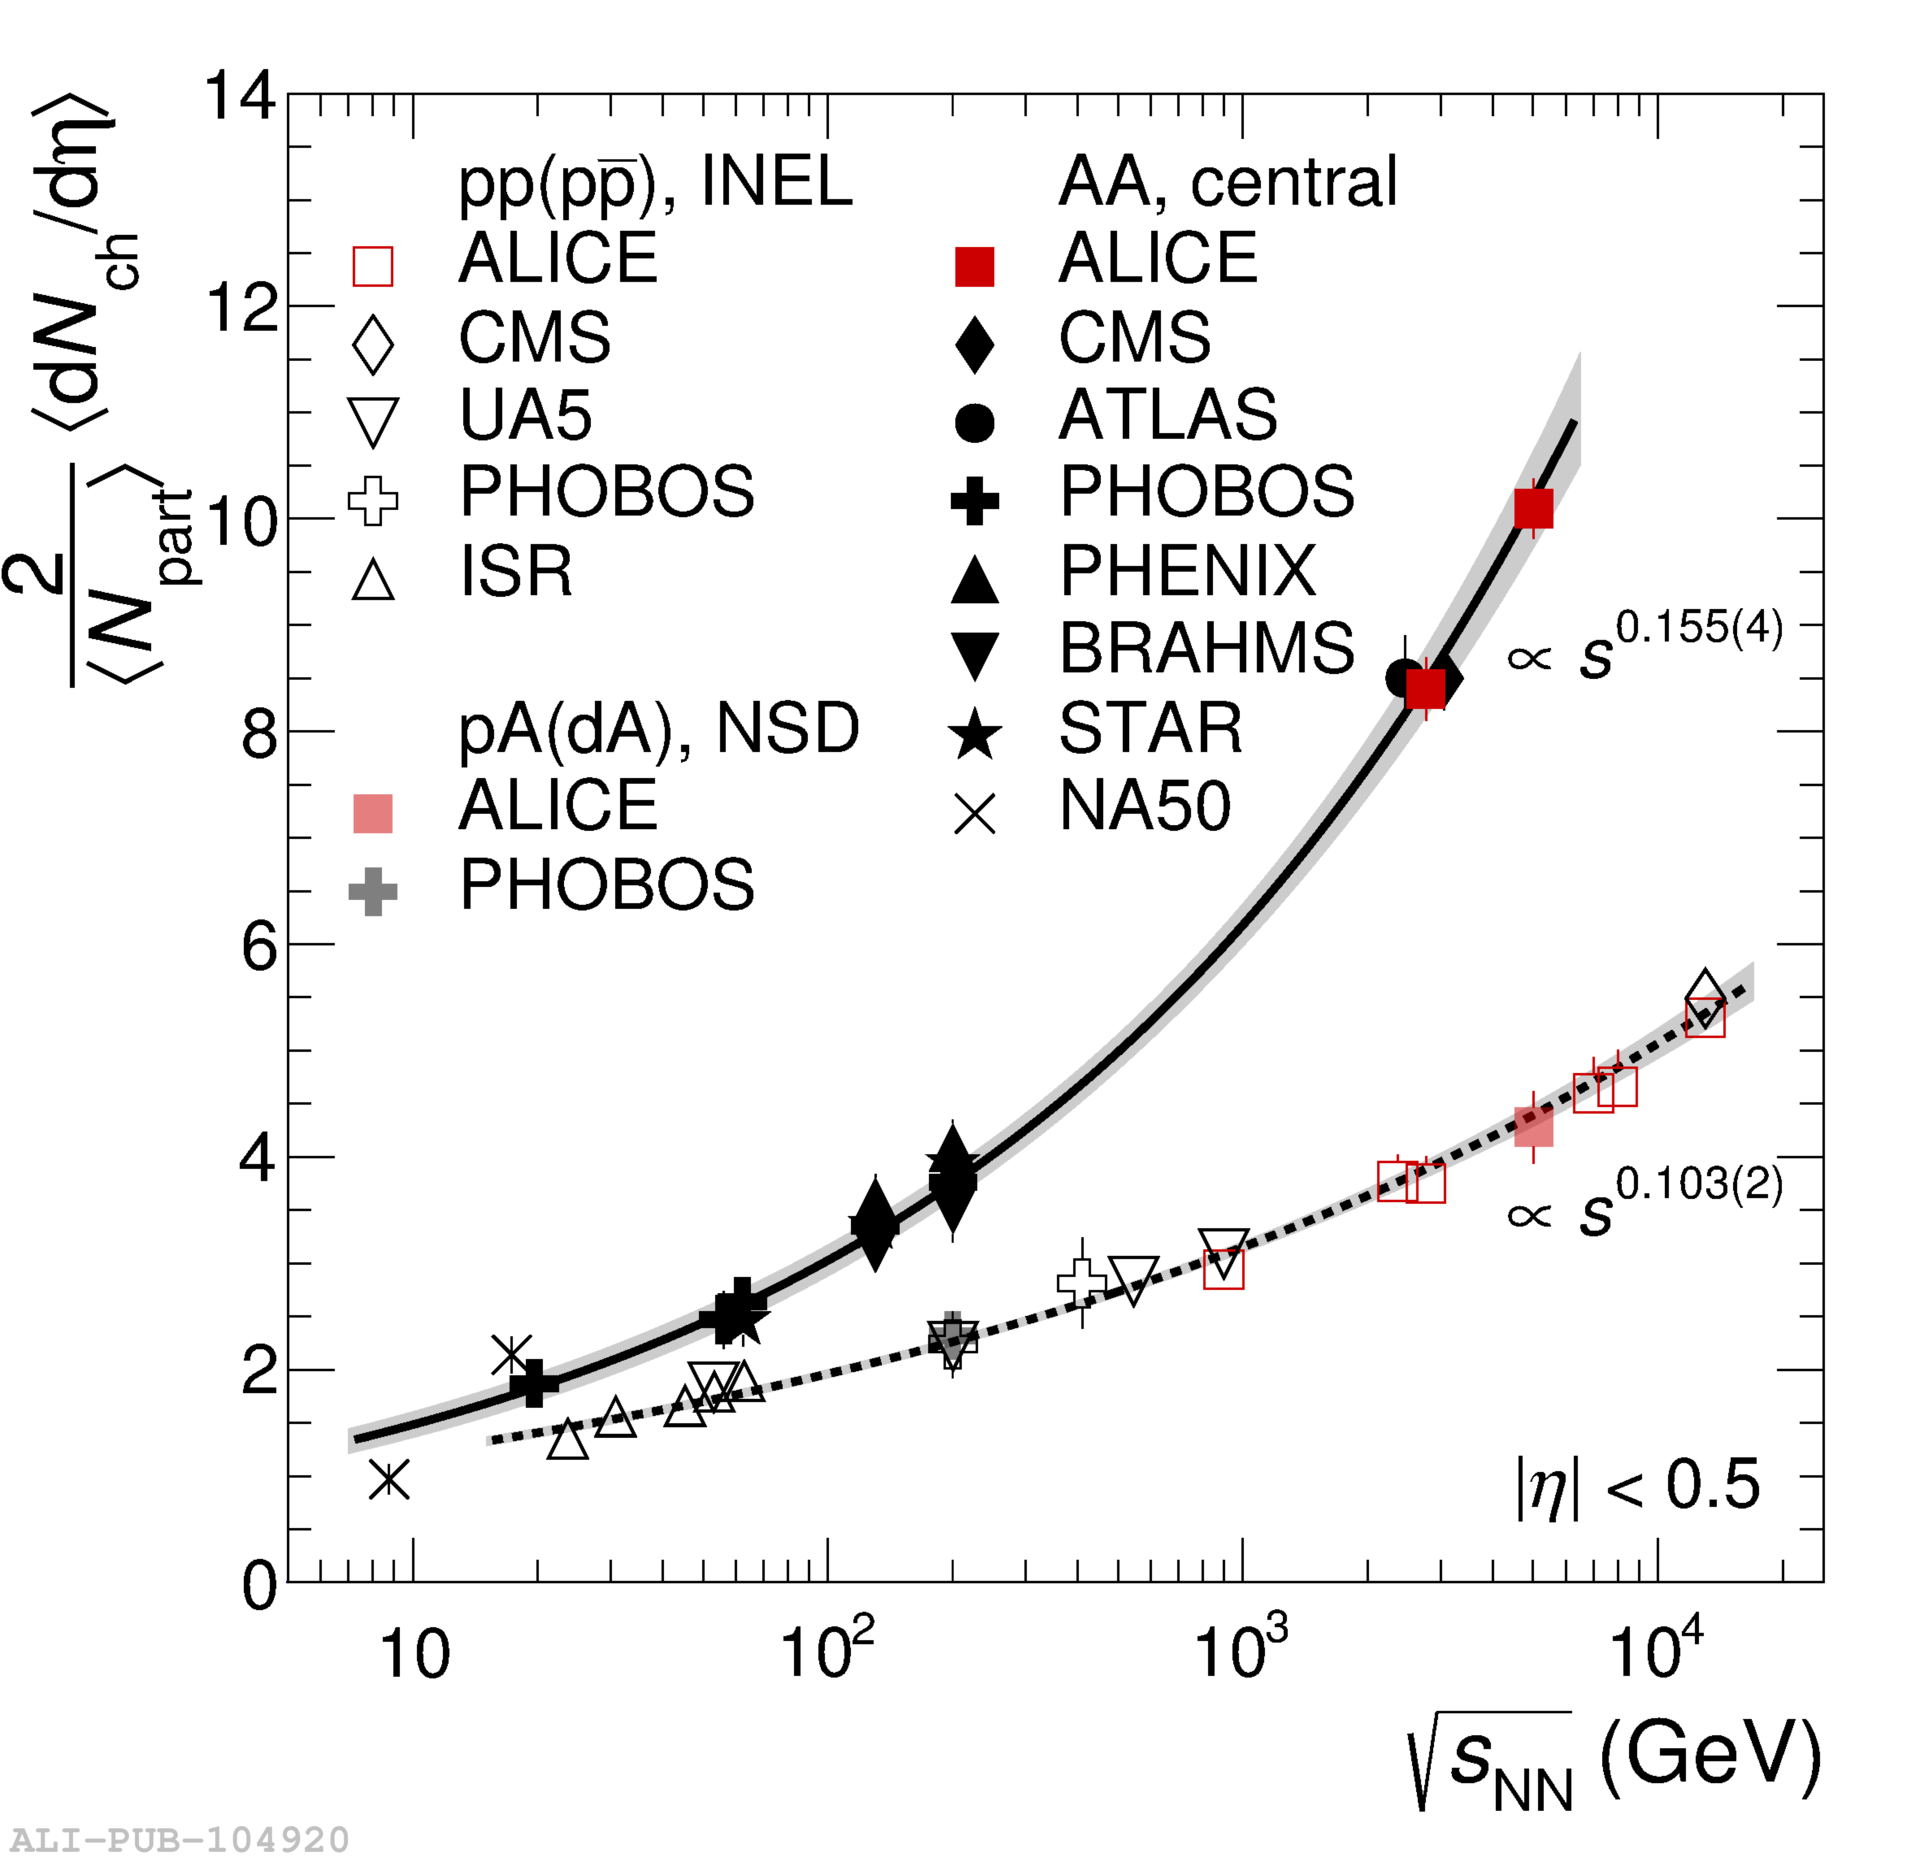
\includegraphics[scale=0.3]{figures/multen.png}\label{fig:multen}}\quad
  \subfloat[][]
  {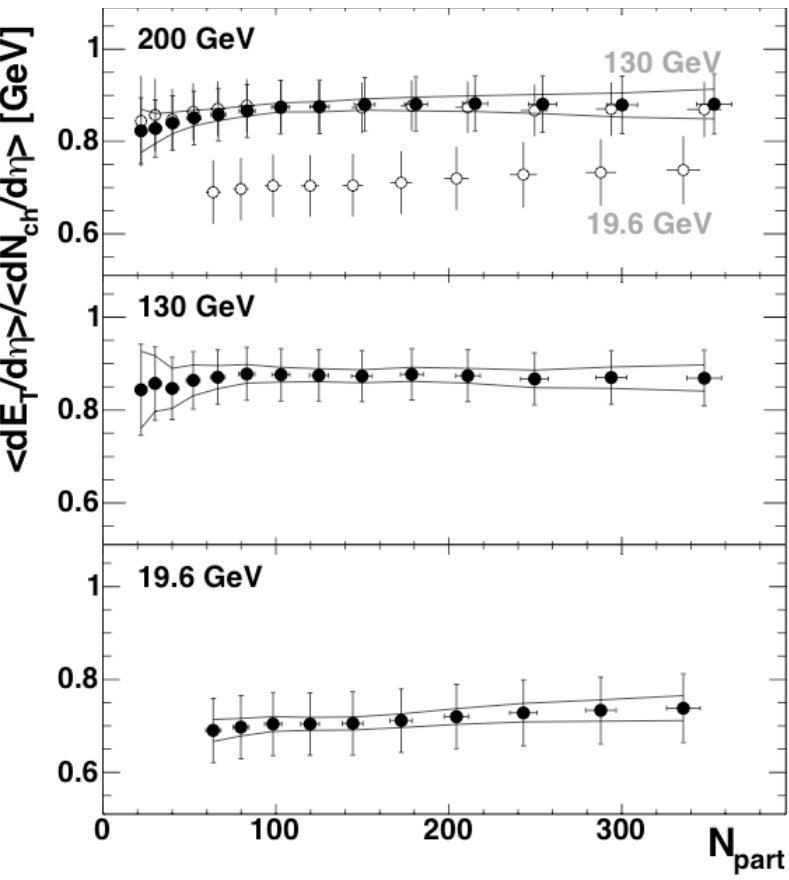
\includegraphics[scale=0.35]{figures/phenix.png}\label{fig:phenix}}
  \caption{(a) Charged pseudorapidity density per participant pair for nucleus-nucleus and p-p collisions, as a function of $\sqrt{s_{NN}}$ \cite{multen}. (b) Ratio between pseudorapidity energy density and pseudorapidity density as a function of the number participants for different values of $\sqrt{s_{NN}}$ at PHENIX experiment.}
\end{figure}
%
In Figure \ref{fig:multen}, the pseudorapidity per participant pair is shown as a function of the energy $\sqrt{s_{NN}}$: the particle production trend is steeper in AA than what obtained in p-p collisions.\\
Then, considering the ratio between the energy pseudorapidity density $\frac{dE}{d\eta}$ and  the pseudorapidity density $\frac{dN}{d\eta}$ as a function of the number of participants, it can be seen that this quantity does not change much with $\sqrt{s_{NN}}$. This means that the extra energy goes into the production of new particles rather than into kinetic energy.\\
\subsubsection{Multiplicity of identified particles}
The measurement of the multiplicity of the hadronic species. i.e. of the chemical composition of the system after the hadronization, allows to get important information about the state of the system at the chemical freeze-out, like, for example, whether the fireball was at the equilibrium or not, the temperature and the baryonic content.\\
The abundances of the different hadronic species produced in an ion collision can be described using the so called \textit{statistical thermal model}, which is based on the hypothesis that the system is at chemical and thermal equilibrium when the chemical freeze-out occurs. With this assumption, it is possible to describe the system using the statistical mechanics, in particular using a grand canonical ensemble with two parameters, the temperature and the baryo-chemical potential. It is important to note that the equilibrium is postulated: this model does not describe the evolution of the collision till the phase transition and not even how this transition takes place. It is a merely statistical equilibrium, due to the way in which the hadronization fills the phase space, realizing the most probable configuration. Secondly, the system is described as an ideal gas of hadrons and resonances (\textit{Hagedorn's gas}, from the name of the scientist who has developed the model). It contains all the degrees of freedom of a strongly interacting confined system, for not too high temperatures (T < 190 MeV). With this method, a gas of interacting hadrons is approximated by a gas of non interacting hadrons and resonances.\\
Using the grand canonical ensemble, the partition function for the gas just described is given by the product of the partition functions of each species:
\begin{equation}
 Z^{GC}(T,V,\mu)\; = \;\prod_{i}Z^{GC}_{i}(T,V,\mu_{i}),
\end{equation}
where, for the left hand side, the chemical potential $\mu$ is the parameter that in the grand canonical ensemble guarantees the average conservation of the quantum numbers:
\begin{equation}
\mu \; = \;\sum_{i} \mu_{Q_{i}}Q_{i},
\end{equation}
where $Q_{i}$ are the conserved quantum numbers, $\mu_{Q_{i}}$ are the chemical potentials associated to these quantities, and $\mu$ is the energy necessary to add to the system a particle with quantum numbers $Q_{i}$.\\
In the case of a gas of particles with a low mass (m < 1.8 GeV), i.e. without heavy quarks, there are three conserved quantum numbers: the third component of the isospin $I_{3}$, the baryonic number \textit{B}, the strangeness \textit{S}. Therefore, for each species $\mu_{i} = \mu_{I_{3}}I_{3i} + \mu_{B}B_{i} + \mu_{S}S_{i}$.
From the definition of the partition function for the single species:
\begin{equation}
 \ln Z_{i}\; = \; \frac{Vg_{i}}{2\pi^{2}}\int_{0}^{\infty}\pm\:p^{2}dp\ln[1\pm e^{-\frac{E-\mu_{i}}{T}}],
\end{equation}
the expression for the density can be derived:
\begin{equation}
n_{i}\; = \; -\frac{T}{V} \frac{\partial \ln Z_{i}}{\partial \mu} \;=\; \frac{g_{i}}{2\pi^{2}} \int_{0}^{\infty}\frac{p^{2}dp}{e^{-\frac{E-\mu_{i}}{T}}\pm1}.
\end{equation}
Finally, from this equation the average multiplicity of a particular species $\langle N_{i} \rangle$ can be easily defined.\\
Thanks to the knowledge of the electric charge, the strangeness and the baryonic number of the initial stage, only three parameters are necessary to estimate the average multiplicity: the temperature, the volume and the baryo-chemical potential. Moreover, if ratios between the multiplicity of different species are used instead of the multiplicity itself, the volume of the system, which is affected by a big uncertainty, is no needed.\\
In conclusion, the temperature and the baryo-chemical potential at the freeze-out can be determined through a $\chi^{2}$ minimization, using:
\begin{equation}
 \chi^{2}\;=\;\sum_{i}\frac{(R_{i}^{exp}-R_{i}^{model})^{2}}{\sigma_{i}^{2}}
\end{equation}
where $R_{i}$ are the ratios just described and $\sigma$ is the error associated to the measurements.\\
Considering the phase diagram, at the LHC the chemical freeze-out is extremely close to the phase transition predicted from the lattice QCD.\\
%
\subsection{Particle momentum spectra and radial flow}
The transverse momentum distributions (or transverse mass distributions) of the particles give an important information about the system created in the heavy ion collision, such as, for example, an estimation of the temperature of the thermal freeze-out. For these reason, there is the necessity to focus on the soft probes, those low transverse momentum particles generated in the last stages of the collision, which constitutes the bulk ($\sim$ 99\%) of the particle yield.\\
From the measurements in p-p collisions, it is known that the transverse mass distributions, normalized to the transverse mass, have an exponential trend:
\begin{equation}
 \frac{1}{m_{T}}\frac{dN}{dm_{T}}\; \propto \; e^{-\frac{m_{T}}{T_{slope}}} \ \ \ \longrightarrow \ \ \ \frac{dN}{dm_{T}}\; \propto \;m_{T}\: e^{-\frac{m_{T}}{T_{slope}}},
\end{equation}
where $T_{slope}$ has the same value for all the particles ($T_{slope} \approx $ 167 MeV).
Experimentally it is easier to measure the transverse momentum instead f the transverse mass, since the latter requires the identification of the particle, but the two distribution are equivalent, due to the easy change of variable:
\begin{equation}
 m_{T}\;=\;\sqrt{m^{2}+p_{T}^2} \ \ \ \longrightarrow \ \ \  p_{T}dp_{T}\;=\;m_{T}dm_{T}.
\end{equation}
Assuming that the observed distributions are thermal Boltzmann distributions, $T_{slope}$ is the temperature at which there is the emission of the particles, i.e. the thermal freeze-out. Hence, $T_{slope} \equiv T_{fo}$\\
%
\begin{figure}
  \centering
  \subfloat[][]
  {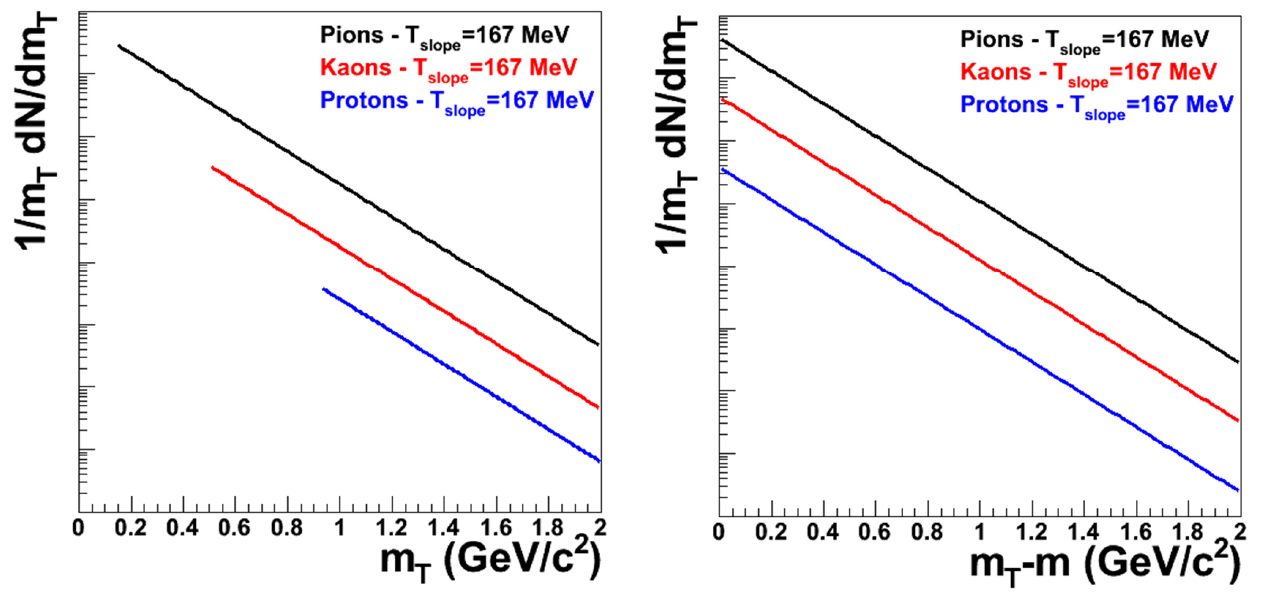
\includegraphics[scale=0.3]{figures/mt.png}\label{fig:mtd}}\quad
  \subfloat[][]
  {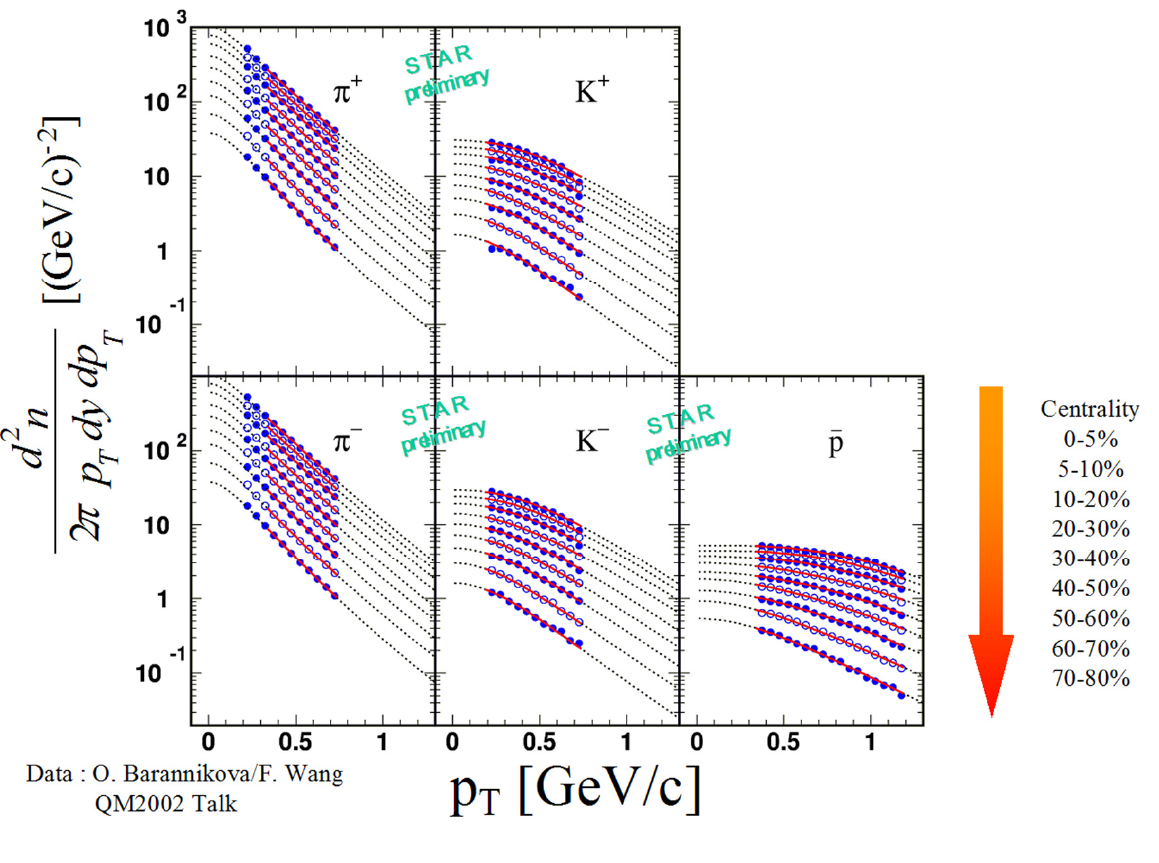
\includegraphics[scale=0.35]{figures/breakscale.png}\label{fig:breakscale}}
  \caption{(a) $m_{T}$ spectra for different particles in p-p collisions. (b) $m_{T}$ spectra for different particles in AA collisions for different values of centrality at the STAR experiment.}
\end{figure}
%
However, in nuclei collisions the $m_{T}$ is broken. In facts, as it can be seen in Figure \ref{fig:breakscale}, the slope of the spectra decreases when the mass of the particle increases, i.e. the heaviest particles are shifted to higher values of $p_{T}$, and $T_{slope}$ has a linear dependence on the mass of the particle. This phenomenon can be explained introducing a collective motion of all the particles, superposed to the thermal motion:
\begin{equation}
 T_{slope}\;=\;T_{fo} + \frac{1}{2}mv_{\perp}^{2}.
\end{equation}
This collective expansion in the transverse plane is called radial flow. This collective motion is generated by the high pressures generated when the nuclear matter is compressed and heated and, in the case of central collisions, this flow is characterized by a circular symmetry on the azimuthal angle in the transverse plane.\\
Fitting the spectra of identified particles, it is possible to separate the thermal component from the collective one, obtaining the freeze-out temperature $T_{fo}$ and the radial speed $\beta_{\perp}$. At the ALICE experiment, the temperature of the thermal freeze-out is $T_{fo} \approx$ 110 - 130 MeV.\\
\subsubsection{Anisotropic flow}
While in central collision the radial flow is characterized by an azimuthal symmetry in the transverse plane, fer semi-central collisions the overlap between the colliding nuclei has an asymmetric almond shape, so the pressure gradients inside the generated medium lead to anisotropies in $\phi$. In facts, the impact parameter generates a favoured direction in the transverse plane: the impact parameter and the beam direction define the so called \textit{reaction plane}, identified by the angle $\Psi_{RP}$ in the transverse plane.\\
%
\begin{figure}
  \centering
  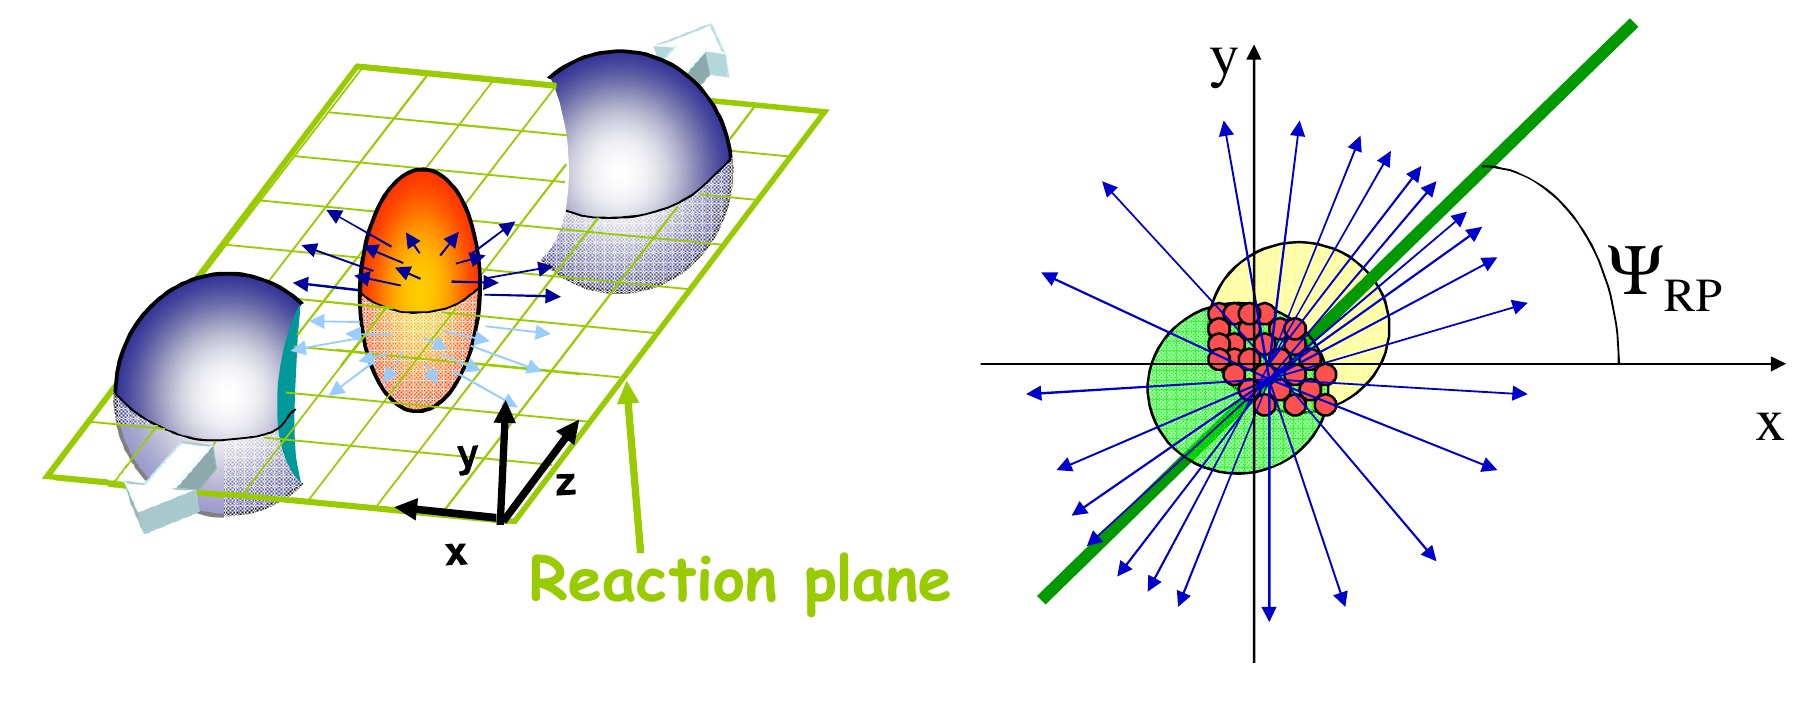
\includegraphics[scale=0.3]{figures/flow.png}
  \caption{Anisotropic flow and reaction plane definition.}
  \label{fig:flow}
\end{figure}
%
There are both spatial anisotropies and momentum anisotropies: the interactions among the particles, if strong enough, can convert the initial geometrical anisotropy into an anisotropy in the momenta distribution, that can be measured.\\
The azimuthal particle distribution can be parametrized with a Fourier expansion:
\begin{equation}
 \frac{dN}{d(\phi-\Psi_{RP})}\;=\;\frac{N_{0}}{2\pi} + \frac{N_{0}}{\pi}\sum_{z} \nu_{k}\cos[k(\phi-\Psi_{RP})]
\end{equation}
In this equation, the sine functions are not present, since the distribution must be symmetric with respect to $\Psi_{RP}$.
The coefficients of the harmonics, which are given by the expression:
\begin{equation}
 \nu_{k}\;=\;\langle \cos[k(\phi-\Psi_{RP})]\rangle,
\end{equation}
describe different kinds of anisotropies: $\nu_{1}$, for example, is the \textit{direct flow} coefficient and describes an asymmetry between forward and backward particle production; $\nu_{2}$, instead, is the elliptic flow, which describes the difference between the number of particle emitted in the reaction plane and in the direction orthogonal to it. For the other coefficients, the situation is similar.\\
The geometrical anisotropy, which is the origin of the elliptic flow, attenuates with the evolution of the system, since the gradients of pressure, which are responsible for this asymmetry, are stronger in the first instants of the collision. Therefore, the measurement of the elliptic flow allows to get information about the state equation of the system in the early stages of the collision, being a good test for hydrodynamic models which describe the evolution of the medium. According to the to the measure of the anisotropic flow, the QGP seems to behave like a perfect fluid, rather than like a perfect gas, as one could expect.\\
\subsection{Nuclear modification factor}
The remaining observables used at the ALICE experiment are hard probes, i.e. particles generated in the first stages of the collision, in processes with an high momentum transfer. For this reason, hard probes can give important information about the properties of the medium, even if they are rare events (< 0.1\%).\\
In order to understand the differences between p-p and nuclei collision, it is important two compare the results of the formers with those of the latters.\\
In nuclei collisions the probability of interaction, according to the Glauber Model, scales with the number of elementary nucleon-nucleon collision $N_{coll}$:
\begin{equation}
 p_{AA}^{hard}\;\propto\;\sigma_{hard}N_{coll}
\end{equation}
For this reason, it is expected that transverse momentum spectra measured in nuclei collision can be obtained scaling the spectra for p-p collisions by the the number of elementary collisions $N_{coll}$.
Therefore, the \textit{nuclear modification factor}  can be defined as:
\begin{equation}
 R_{AA}(p_{T})\;=\;\frac{1}{\langle N_{coll}\rangle}\frac{dN_{AA}/dp_{T}}{dN_{pp}/dp_{T}}.
\end{equation}
For low values of the transverse momentum ($p_{T} \lesssim$ 2 GeV), $R_{AA}$ < 1 is expected, since the probability for soft processes, according to the Glauber model, scales with the number of participants $N_{part}$. For hard particles, instead, $R_{AA} \sim$ 1 is expected. It is important to note that heavy quarks (c, b, t) belong to hard physics independently from the transverse momentum value, because their high masses can be produced only in processes with a high momentum transfer. In reality, for values of $p_{T} \gtrsim$ 2 GeV, the $R_{AA}$ is greater than the unity, thanks to phenomena like the Cronin effect, i.e. a translation of the $p_{T}$ spectra towards higher values, due to multiple interactions of the nucleon inside the other nucleus, and the modification of the parton distribution functions. These are called initial states effects because they are not influenced by the evolution of the system, but depend on initial conditions. The $R_{AA}$ can also be modified by final state effects, which reflect the interaction of the particles with the medium generated in the collision. Indeed, since high momentum partons are created in the first stages of the collision, they undergo all the evolution of the collision and their momentum can change due to the energy loss in the fireball, which could lead to the quenching of high $p_{T}$ spectra. The energy loss can be evaluated from the \textit{BDMPS formula}[da mettere]:
\begin{equation}
 \langle \Delta E \rangle \;\propto\;\alpha_{S} \:C_{R}\: \hat{q}\: L^{2},
\end{equation}
where $\alpha_{S}$ is the QCD coupling constant, $C_{R}$ is the Casimir factor, whose value is 4/3 for a quark-gluon coupling and 3 for a gluon-gluon 
one, $\hat{q}$ is the transport coefficient, related to the properties of the medium and proportional to the density and the momenta of the gluons. \textit{L}, finally, is the distance travelled by the particle in the medium. This formula parametrizes the energy loss through the emission of gluons and this gives an explanation of the dependence from $L^{2}$, since the gluons can also interact with the medium.\\
In the next sections, the main hard probes observed at ALICE will be described.\\
\subsection{Jet quenching}
A jet is a collimated emission of hadrons, which originates from fragmentation of a high-$p_{T}$ parton. These partons are created back to back in the initial collision and they form hadrons during the hadronization. For this reason, in small systems, such as in p-p collisions, two jets of hadrons emitted in opposite directions are usually seen. In ion collisions, however, the situation in different, since the high energy parton can interact with the medium and, consequently, lose energy as previously described.
%
\begin{figure}
  \centering
  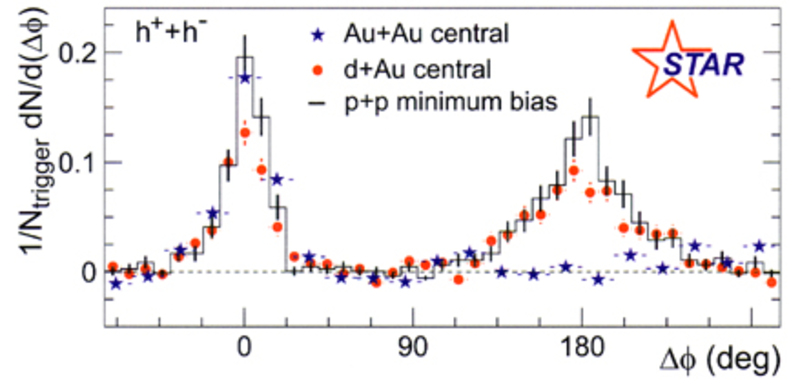
\includegraphics[scale=0.3]{figures/zoom.jpeg}
  \caption{Azimuthal distributions for p-p, d-Au, Au-Au at STAR \cite{jets}.}
  \label{fig:jet}
\end{figure}
%
Hence, for ion collisions, the azimuthal distribution of high momentum particles is strongly dependent on the point of creation of the pair $q\bar{q}$. Indeed, if the partons are produced inside the fireball, they are slowed down while exiting the medium and so they hadronize in low $p_{T}$ particles. Otherwise, if the pair is produced on the surface of the fireball, the hadron whose momentum is directed outwards hadronizes in a high $p_{T}$ particle, i.e. creates a jet that can be detected, while the parton emitted inwards travels through the whole fireball, losing energy and hadronizing in a low $p_{T}$ particle. Therefore, the study of azimuthal angle correlation between two high $p_{T}$ particles can give important information about the creation of a hot and dense medium.\\
In Figure \ref{fig:jet}, the measures of the azimuthal correlation are reported for p-p, d-Au and Au-AU collisions for the STAR experiment. As it can be seen, for the first two kinds of collision there are two jets emitted back to back, while for heavy ions collisions one of the jets is suppressed. This can be considered a proof of the creation of a hot and dense medium, such as the QGP.\\
\subsection{Open heavy flavours}
Particles constituted by a heavy quark, i.e. charm and beauty, are called \textit{open heavy flavours}. Considering the great mass value of the heavy quarks ($m_{b}\sim$ 4.8 GeV and $m_{c}\sim$ 1.2 GeV), they can only be produced in the initial stages of the collision, in scatterings with a high momentum transfer between partons. For this reason, their production con be described using the perturbative QCD till very low values of transverse momentum. This kind of measurements is used both in p-p collisions, in order to test the theoretical model based on the perturbative QCD and to have a reference for the $R_{AA}$ determination, and in heavy ion collisions, in order to test the energy loss models.\\
In particular, the energy loss models predict a different loss for hadrons containing heavy quarks compared to light hadrons. This is explained with the different origin of the two types: heavy flavours are generated from a quark fragmentation, while light flavours are mainly produced from gluons. Then, the is the so called \textit{dead cone effect} \cite{deadcone}: the gluon radiation is suppressed at small angles (with respect to the direction of motion) for heavy quarks. In particular, being $E_{Q}$ and $M_{Q}$ respectively the energy and the mass of the heavy quark, the suppression is predicted for angles $\theta<\frac{M_{Q}}{E_{Q}}$. Therefore, the energy loss for light flavours is bigger than in heavy flavours, and the energy loss loss of a particle with a charm quark is bigger than that of a particle with a beauty. The measures of $R_{AA}$ seem to confirm this behaviour for charmed and beautied particles, but higher statistics is needed in order to see the difference between charmed particles and light flavours.\\
\subsection{Heavy quarkonia suppression}
Another hard probe of the QGP is given by the heavy quarkonia, i.e. bound states made of a heavy quark and the respective antiquark: charmonium ($c\bar{c}$) and bottomonium ($b\bar{b}$). Since they are composed of heavy quarks, they have been generated in the first stages of the collision. However, the quarks in this bound states are characterized by a non relativistic motion ($\beta\sim$ 0.4) and so the system cannot be described using a perturbative approach.\\
In the vacuum, the binding potential of a quarkonium state can be expressed using the Cornell potential:
\begin{equation}
 V(r)\;=\;-\frac{\alpha_{S}}{r}+kr,
\end{equation}
where \textit{k} is a parameter and \textit{r} is he distance between \textit{q} and $\bar{q}$.
As it can be seen, this potential is composed of a coulombian potential, induce by the exchange of a gluon, and a confining potential, which parametrizes the non perturbative effects.\\
However, if the quarkonium is immersed in the QGP, the binding potential changes, since the presence of free quarks and gluons act as a screen bewteen the pair $q\bar{q}$. Therefore, in this case the potential becomes a Yukawa type potential:
\begin{equation}
 V(r)\;=\;-\frac{\alpha_{S}}{r}e^{-\frac{r}{\lambda_{D}}}.
\end{equation}
The quantity $\lambda_{D}$ is called \textit{Debye length}, and is related to the the longest distance at which two colour charges can form a bound state in a QGP. An expression for the Debye length can be obtained from leading order calculations in perturbative QCD:
\begin{equation}
 \lambda_{D}\;=\;\frac{1}{g\sqrt{\frac{N_{c}}{3}+\frac{N_{f}}{6}}T},
\end{equation}
where $N_{c}$ is the number of colours and $N_{f}$ is the number of flavours.\
The Debye length, hence, decreases when the temperature increases and, consequently, it is possible to determine the temperature of the QGP from the presence or the suppression of a particular excited state of quarkonia. In facts, states which are more bounded have smaller dimensions and, for this reason, they survive at higher temperatures.\\
The idea of using the $J/\Psi$ suppression as a signature of the QGP formation was introduced in 1986 by Matsui and Satz, in one of the most famous articles of the ultra-relativistic ion physics \cite{matsui}.\\
%
\begin{figure}
  \centering
  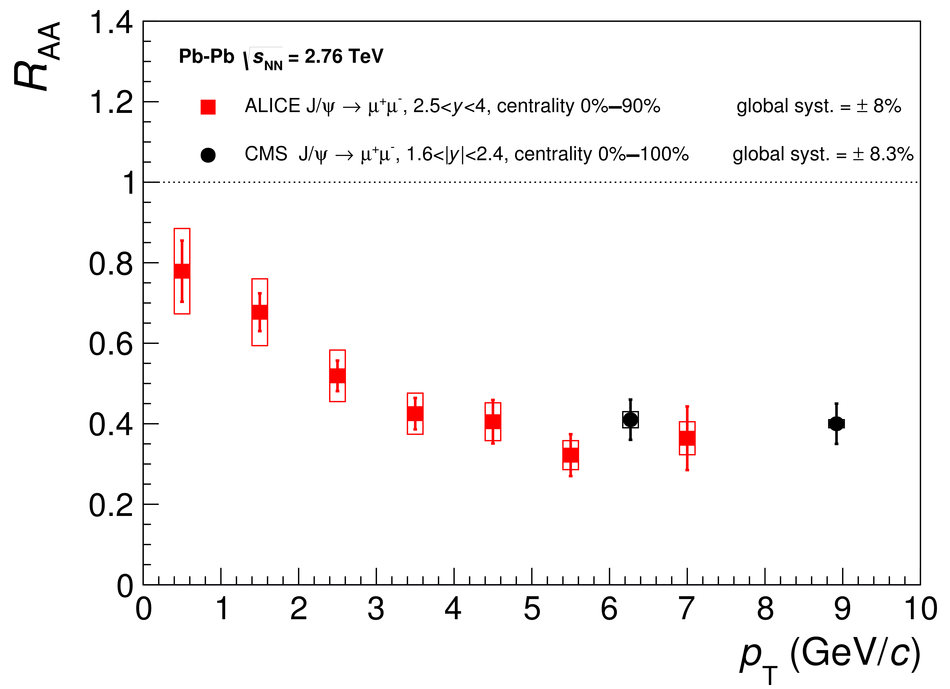
\includegraphics[scale=0.25]{figures/jpsi.png}
  \caption{Transverse momentum dependence of the centrality integrated $J/\Psi$ $R_{AA}$ measured by ALICE in Pb-Pb collisions at $\sqrt{s_{NN}}$ = 2.76 GeV compared to CMS results at the same $\sqrt{s_{NN}}$.}
  \label{fig:jpsi}
\end{figure}
%

\printbibliography


\end{document}          
